\documentclass{standalone}
\usepackage{tikz}
\usetikzlibrary{patterns, positioning}


\begin{document}
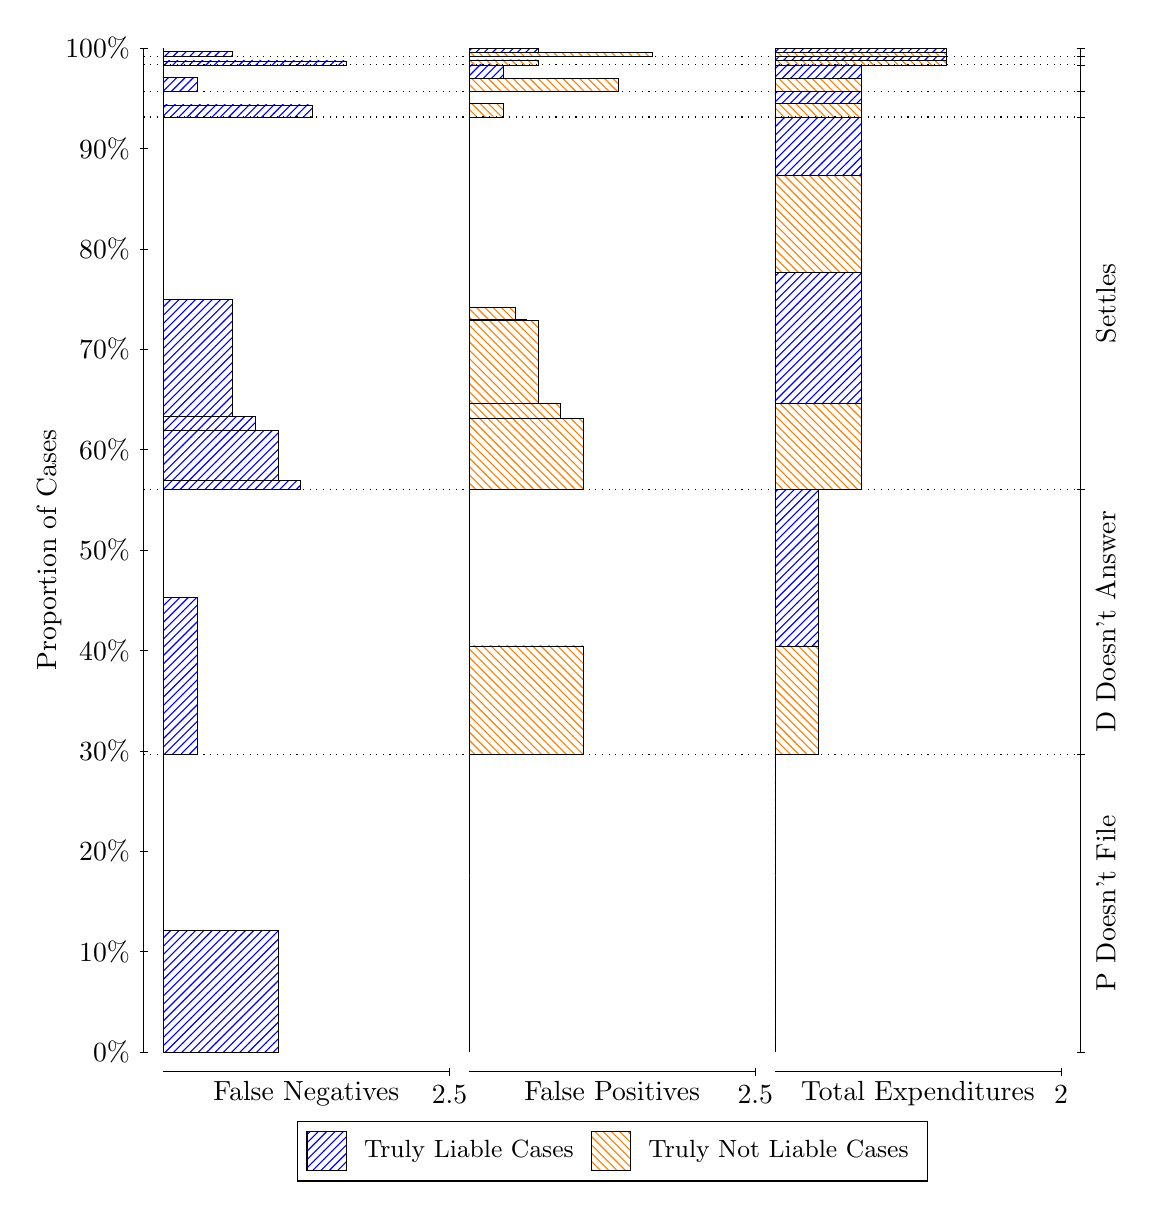
\begin{tikzpicture}
\draw[black, very thin] (1.5,1.75) -- (1.5,14.5);
\node[rotate=90, text=black, anchor=center] at (0.3, 8.125) {Proportion of Cases};
\draw[black, very thin] (1.45,1.75) -- (1.55,1.75);
\node[text=black, anchor=east] at (1.45, 1.75) {0\%};
\draw[black, very thin] (1.45,3.025) -- (1.55,3.025);
\node[text=black, anchor=east] at (1.45, 3.025) {10\%};
\draw[black, very thin] (1.45,4.3) -- (1.55,4.3);
\node[text=black, anchor=east] at (1.45, 4.3) {20\%};
\draw[black, very thin] (1.45,5.575) -- (1.55,5.575);
\node[text=black, anchor=east] at (1.45, 5.575) {30\%};
\draw[black, very thin] (1.45,6.85) -- (1.55,6.85);
\node[text=black, anchor=east] at (1.45, 6.85) {40\%};
\draw[black, very thin] (1.45,8.125) -- (1.55,8.125);
\node[text=black, anchor=east] at (1.45, 8.125) {50\%};
\draw[black, very thin] (1.45,9.4) -- (1.55,9.4);
\node[text=black, anchor=east] at (1.45, 9.4) {60\%};
\draw[black, very thin] (1.45,10.675) -- (1.55,10.675);
\node[text=black, anchor=east] at (1.45, 10.675) {70\%};
\draw[black, very thin] (1.45,11.95) -- (1.55,11.95);
\node[text=black, anchor=east] at (1.45, 11.95) {80\%};
\draw[black, very thin] (1.45,13.225) -- (1.55,13.225);
\node[text=black, anchor=east] at (1.45, 13.225) {90\%};
\draw[black, very thin] (1.45,14.5) -- (1.55,14.5);
\node[text=black, anchor=east] at (1.45, 14.5) {100\%};

\draw[black, very thin] (13.4,1.75) -- (13.4,14.5);
\draw[black, very thin] (13.35,1.75) -- (13.45,1.75);
\node[anchor=west] at (13.35, 1.75) {};
\draw[black, very thin] (13.35,5.5288) -- (13.45,5.5288);
\node[anchor=west] at (13.35, 5.5288) {};
\draw[black, very thin] (13.35,8.8961) -- (13.45,8.8961);
\node[anchor=west] at (13.35, 8.8961) {};
\draw[black, very thin] (13.35,13.624) -- (13.45,13.624);
\node[anchor=west] at (13.35, 13.624) {};
\draw[black, very thin] (13.35,13.953) -- (13.45,13.953);
\node[anchor=west] at (13.35, 13.953) {};
\draw[black, very thin] (13.35,14.287) -- (13.45,14.287);
\node[anchor=west] at (13.35, 14.287) {};
\draw[black, very thin] (13.35,14.398) -- (13.45,14.398);
\node[anchor=west] at (13.35, 14.398) {};
\draw[black, very thin] (13.35,14.5) -- (13.45,14.5);
\node[anchor=west] at (13.35, 14.5) {};

\draw[black, very thin, pattern color=blue, pattern=north east lines] (1.75,1.75) rectangle (3.2033,3.2895);
\draw[black, very thin, pattern color=orange, pattern=north west lines] (1.75,3.2895) rectangle (1.75,5.5288);
\draw[black, very thin, pattern color=blue, pattern=north east lines] (1.75,5.5288) rectangle (2.186,7.5186);
\draw[black, very thin, pattern color=orange, pattern=north west lines] (1.75,7.5186) rectangle (1.75,8.8961);
\draw[black, very thin, pattern color=blue, pattern=north east lines] (1.75,8.8961) rectangle (3.494,9.0068);
\draw[black, very thin, pattern color=blue, pattern=north east lines] (1.75,9.0068) rectangle (3.3487,9.0129);
\draw[black, very thin, pattern color=blue, pattern=north east lines] (1.75,9.0129) rectangle (3.2033,9.6429);
\draw[black, very thin, pattern color=blue, pattern=north east lines] (1.75,9.6429) rectangle (2.9127,9.8239);
\draw[black, very thin, pattern color=blue, pattern=north east lines] (1.75,9.8239) rectangle (2.622,11.31);
\draw[black, very thin, pattern color=orange, pattern=north west lines] (1.75,11.31) rectangle (1.75,13.624);
\draw[black, very thin, pattern color=blue, pattern=north east lines] (1.75,13.624) rectangle (3.6393,13.779);
\draw[black, very thin, pattern color=orange, pattern=north west lines] (1.75,13.779) rectangle (1.75,13.953);
\draw[black, very thin, pattern color=blue, pattern=north east lines] (1.75,13.953) rectangle (2.186,14.125);
\draw[black, very thin, pattern color=orange, pattern=north west lines] (1.75,14.125) rectangle (1.75,14.287);
\draw[black, very thin, pattern color=blue, pattern=north east lines] (1.75,14.287) rectangle (4.0753,14.336);
\draw[black, very thin, pattern color=orange, pattern=north west lines] (1.75,14.336) rectangle (1.75,14.398);
\draw[black, very thin, pattern color=blue, pattern=north east lines] (1.75,14.398) rectangle (2.622,14.454);
\draw[black, very thin, pattern color=orange, pattern=north west lines] (1.75,14.454) rectangle (1.75,14.5);
\draw[black, very thin, pattern color=orange, pattern=north west lines] (5.6333,1.75) rectangle (5.6333,3.9893);
\draw[black, very thin, pattern color=blue, pattern=north east lines] (5.6333,3.9893) rectangle (5.6333,5.5288);
\draw[black, very thin, pattern color=orange, pattern=north west lines] (5.6333,5.5288) rectangle (7.0867,6.9064);
\draw[black, very thin, pattern color=blue, pattern=north east lines] (5.6333,6.9064) rectangle (5.6333,8.8961);
\draw[black, very thin, pattern color=orange, pattern=north west lines] (5.6333,8.8961) rectangle (7.0867,9.7951);
\draw[black, very thin, pattern color=orange, pattern=north west lines] (5.6333,9.7951) rectangle (6.796,9.984);
\draw[black, very thin, pattern color=orange, pattern=north west lines] (5.6333,9.984) rectangle (6.5053,11.043);
\draw[black, very thin, pattern color=orange, pattern=north west lines] (5.6333,11.043) rectangle (6.36,11.051);
\draw[black, very thin, pattern color=orange, pattern=north west lines] (5.6333,11.051) rectangle (6.2147,11.21);
\draw[black, very thin, pattern color=blue, pattern=north east lines] (5.6333,11.21) rectangle (5.6333,13.624);
\draw[black, very thin, pattern color=orange, pattern=north west lines] (5.6333,13.624) rectangle (6.0693,13.799);
\draw[black, very thin, pattern color=blue, pattern=north east lines] (5.6333,13.799) rectangle (5.6333,13.953);
\draw[black, very thin, pattern color=orange, pattern=north west lines] (5.6333,13.953) rectangle (7.5227,14.115);
\draw[black, very thin, pattern color=blue, pattern=north east lines] (5.6333,14.115) rectangle (6.0693,14.287);
\draw[black, very thin, pattern color=orange, pattern=north west lines] (5.6333,14.287) rectangle (6.5053,14.35);
\draw[black, very thin, pattern color=blue, pattern=north east lines] (5.6333,14.35) rectangle (5.6333,14.398);
\draw[black, very thin, pattern color=orange, pattern=north west lines] (5.6333,14.398) rectangle (7.9587,14.444);
\draw[black, very thin, pattern color=blue, pattern=north east lines] (5.6333,14.444) rectangle (6.5053,14.5);
\draw[black, very thin, pattern color=orange, pattern=north west lines] (9.5167,1.75) rectangle (9.5167,3.9893);
\draw[black, very thin, pattern color=blue, pattern=north east lines] (9.5167,3.9893) rectangle (9.5167,5.5288);
\draw[black, very thin, pattern color=orange, pattern=north west lines] (9.5167,5.5288) rectangle (10.062,6.9064);
\draw[black, very thin, pattern color=blue, pattern=north east lines] (9.5167,6.9064) rectangle (10.062,8.8961);
\draw[black, very thin, pattern color=orange, pattern=north west lines] (9.5167,8.8961) rectangle (10.607,9.984);
\draw[black, very thin, pattern color=blue, pattern=north east lines] (9.5167,9.984) rectangle (10.607,11.652);
\draw[black, very thin, pattern color=orange, pattern=north west lines] (9.5167,11.652) rectangle (10.607,12.878);
\draw[black, very thin, pattern color=blue, pattern=north east lines] (9.5167,12.878) rectangle (10.607,13.624);
\draw[black, very thin, pattern color=orange, pattern=north west lines] (9.5167,13.624) rectangle (10.607,13.799);
\draw[black, very thin, pattern color=blue, pattern=north east lines] (9.5167,13.799) rectangle (10.607,13.953);
\draw[black, very thin, pattern color=orange, pattern=north west lines] (9.5167,13.953) rectangle (10.607,14.115);
\draw[black, very thin, pattern color=blue, pattern=north east lines] (9.5167,14.115) rectangle (10.607,14.287);
\draw[black, very thin, pattern color=orange, pattern=north west lines] (9.5167,14.287) rectangle (11.697,14.35);
\draw[black, very thin, pattern color=blue, pattern=north east lines] (9.5167,14.35) rectangle (11.697,14.398);
\draw[black, very thin, pattern color=orange, pattern=north west lines] (9.5167,14.398) rectangle (11.697,14.444);
\draw[black, very thin, pattern color=blue, pattern=north east lines] (9.5167,14.444) rectangle (11.697,14.5);
\draw[black, dotted] (1.5,5.5288) -- (13.4,5.5288);
\draw[black, dotted] (1.5,8.8961) -- (13.4,8.8961);
\draw[black, dotted] (1.5,13.624) -- (13.4,13.624);
\draw[black, dotted] (1.5,13.953) -- (13.4,13.953);
\draw[black, dotted] (1.5,14.287) -- (13.4,14.287);
\draw[black, dotted] (1.5,14.398) -- (13.4,14.398);
\draw[black, very thin] (1.75,1.5) -- (5.3833,1.5);
\node[text=black, anchor=north] at (3.5667, 1.5) {False Negatives};
\draw[black, very thin] (5.3833,1.45) -- (5.3833,1.55);
\node[text=black, anchor=north] at (5.3833, 1.45) {2.5};

\draw[black, very thin] (5.6333,1.5) -- (9.2667,1.5);
\node[text=black, anchor=north] at (7.45, 1.5) {False Positives};
\draw[black, very thin] (9.2667,1.45) -- (9.2667,1.55);
\node[text=black, anchor=north] at (9.2667, 1.45) {2.5};

\draw[black, very thin] (9.5167,1.5) -- (13.15,1.5);
\node[text=black, anchor=north] at (11.333, 1.5) {Total Expenditures};
\draw[black, very thin] (13.15,1.45) -- (13.15,1.55);
\node[text=black, anchor=north] at (13.15, 1.45) {2};

\node[text=black, centered, rotate=90] at (13.72, 3.6394) {P Doesn't File};
\node[text=black, centered, rotate=90] at (13.72, 7.2125) {D Doesn't Answer};
\node[text=black, centered, rotate=90] at (13.72, 11.26) {Settles};





\draw (7.449999999999999,1.5) node[draw=none] (baseCoordinate) {};
\begin{scope}[align=center]
        \matrix[scale=0.5, draw=black, below=0.5cm of baseCoordinate, nodes={draw}, column sep=0.1cm]{
            \node[rectangle, draw, minimum width=0.5cm, minimum height=0.5cm, pattern color=blue, pattern=north east lines] {}; &
            \node[draw=none, font=\small, text=black] (B) {Truly Liable Cases}; &
            \node[rectangle, draw, minimum width=0.5cm, minimum height=0.5cm, pattern color=orange, pattern=north west lines] {}; &
            \node[draw=none, font=\small, text=black] (B) {Truly Not Liable Cases}; \\
            };
\end{scope}

\end{tikzpicture}
\end{document}